\documentclass[12pt]{scrartcl}

\usepackage[utf8]{inputenc}
\usepackage[naustrian]{babel}
\usepackage{caption}
\usepackage{graphicx}
\usepackage{verbatim}
\usepackage[T1]{fontenc}
\usepackage{lmodern}
\usepackage{subcaption}
\usepackage{amsfonts}
\usepackage{listings}
\usepackage{float}

%pdfs
\usepackage{pdfpages}
\usepackage{tikz}

%page borders
\usepackage{geometry}
\geometry{left=2.5cm,right=2.5cm,top=3cm,bottom=2.5cm}

\usepackage{minted}
\setminted {
	%style=igor, %borland, autumn, vs
	encoding=utf-8,
	autogobble,
	tabsize=4,
	linenos,
	breaklines,
	keywordcase=upper,
	%escapeinside=||
	%bgcolor=bg
	%frame=single
}

\newenvironment{code}{\captionsetup{type=listing}}{}

%title/footer/header values
\usepackage{titling}
\title{DES3UE Übung 5}
\author{Elias Leonhardsberger}
\date{\today{}, Hagenberg}

%footer/header
%\usepackage[automark]{scrpage2}
%\pagestyle{headings}
%\clearscrheadfoot
%\ihead{\thetitle}
%\chead{\theauthor}
%\ohead{\today}
%\cfoot{Seite \pagemark}

\begin{document}
\clearpage
\thispagestyle{empty}
\begin{tikzpicture}[remember picture, overlay]
	\node at (current page.center) {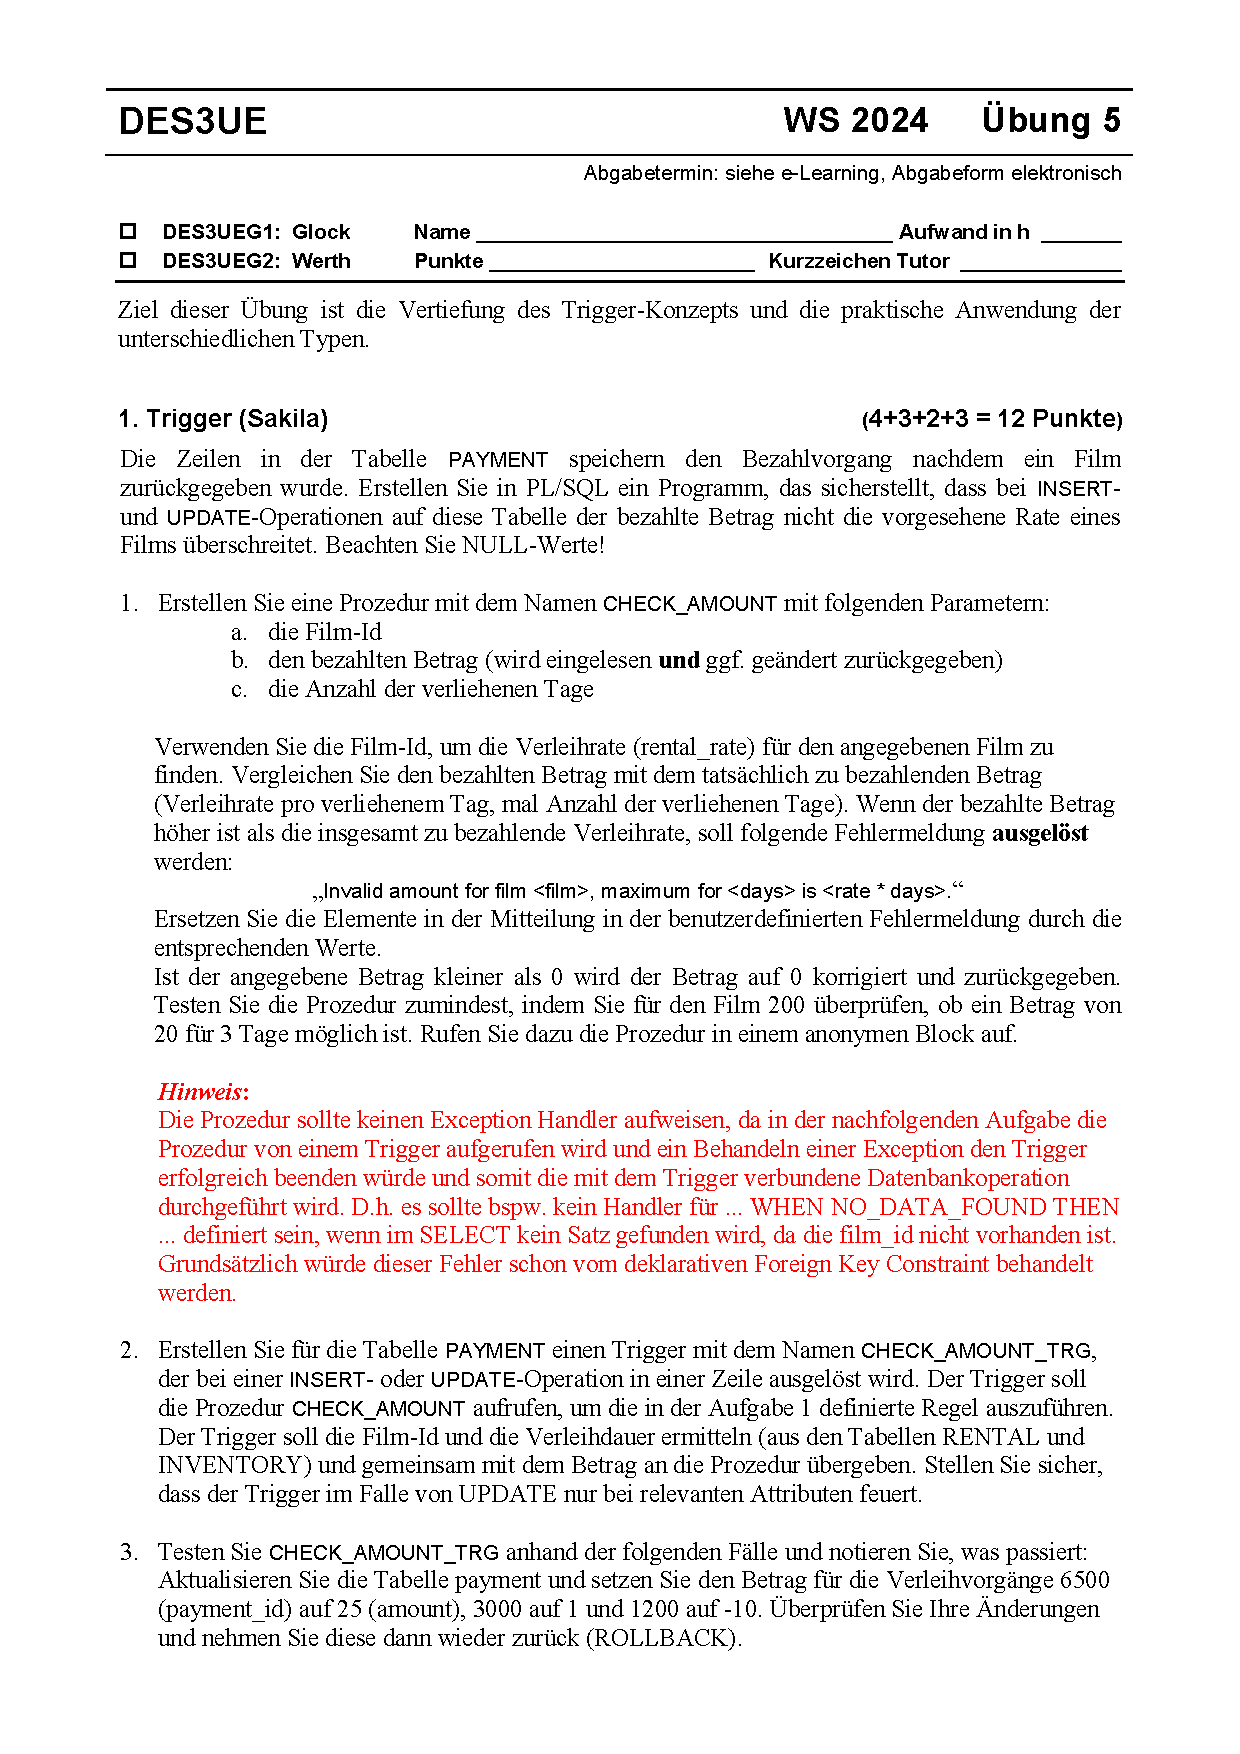
\includegraphics[page=1]{Angabe.pdf}};
	\begin{scope}[shift={(current page.south west)},every node/.style={anchor=base west}]
		\node at (1.87cm, 25.65cm) {X};
		\node at (8.5cm, 25.75cm) {\theauthor};
		\node at (17.7cm, 25.75cm) {4};
	\end{scope}
\end{tikzpicture}

\includepdf[pages=2-3]{Angabe.pdf}

\maketitle
\tableofcontents

\pagebreak

% 1_1.png    1_3_2.png  1_3_4.png  1_3_6.png  1_4_2.png  1_4_4.png  2_3_1.png  2_3_3.png  2_3_5.png  2_3_7.png  latex	%ue5_1_2.sql  ue5_1_4.sql  ue5_2_2.sql  ue5_2.sql    ue5_3_2.sql
% 1_3_1.png  1_3_3.png  1_3_5.png  1_4_1.png  1_4_3.png  1_4_5.png  2_3_2.png  2_3_4.png  2_3_6.png  3_2.png    ue5_1_1.sql  ue5_1_3.sql  ue5_2_1.sql  ue5_2_3.sql  ue5_3_1.sql

\section{Trigger (Sakila)}

\subsection{SQL-Statements}

\subsubsection{Aufgabe 1}
\inputminted{sql}{../ue5_1_1.sql}

\subsubsection{Aufgabe 2}
\inputminted{sql}{../ue5_1_2.sql}

\subsubsection{Aufgabe 3}
\inputminted{sql}{../ue5_1_3.sql}

\subsubsection{Aufgabe 4}
\inputminted{sql}{../ue5_1_4.sql}

\subsection{Ergebnisse}

\begin{figure}[H]
	\centering
	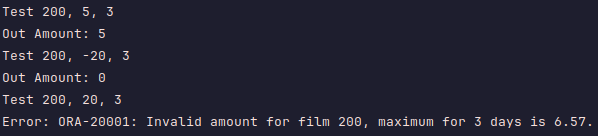
\includegraphics[width=0.8\textwidth]{../1_1.png}
	\caption{Ausgabe 1\textunderscore1}
\end{figure}

\pagebreak

\begin{figure}[H]
	\centering
	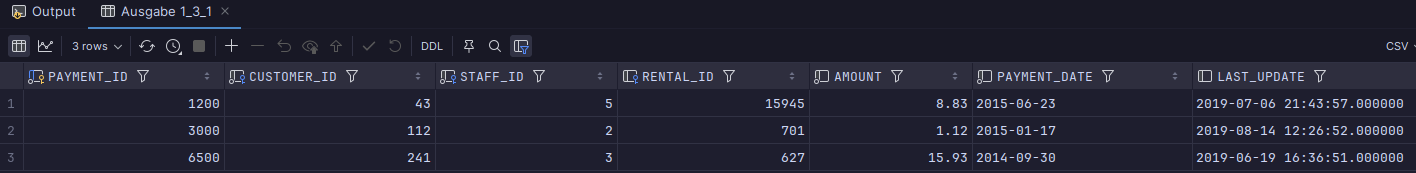
\includegraphics[width=1\textwidth]{../1_3_1.png}
	\caption{Ausgabe 1\textunderscore3\textunderscore1}
\end{figure}

\begin{figure}[H]
	\centering
	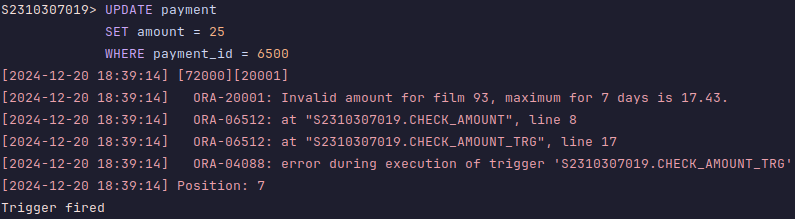
\includegraphics[width=0.8\textwidth]{../1_3_2.png}
	\caption{Ausgabe 1\textunderscore3\textunderscore2}
\end{figure}

\begin{figure}[H]
	\centering
	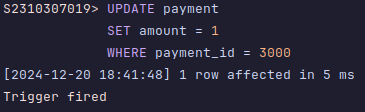
\includegraphics[width=0.4\textwidth]{../1_3_3.png}
	\caption{Ausgabe 1\textunderscore3\textunderscore3}
\end{figure}

\begin{figure}[H]
	\centering
	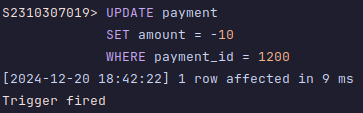
\includegraphics[width=0.4\textwidth]{../1_3_4.png}
	\caption{Ausgabe 1\textunderscore3\textunderscore4}
\end{figure}

\begin{figure}[H]
	\centering
	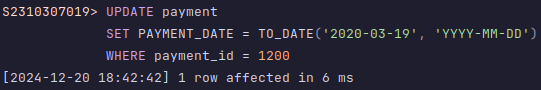
\includegraphics[width=0.7\textwidth]{../1_3_5.png}
	\caption{Ausgabe 1\textunderscore3\textunderscore5}
\end{figure}

\begin{figure}[H]
	\centering
	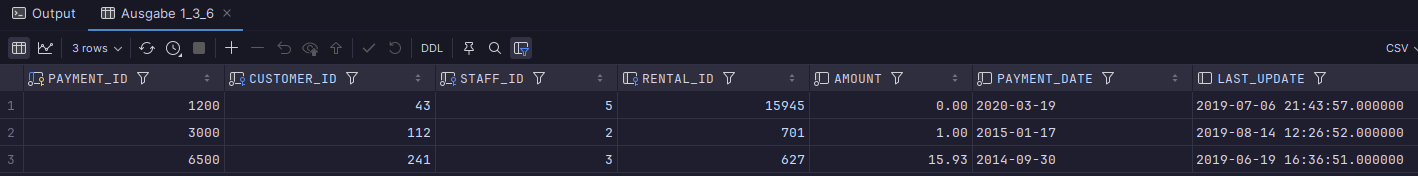
\includegraphics[width=1\textwidth]{../1_3_6.png}
	\caption{Ausgabe 1\textunderscore3\textunderscore6}
\end{figure}

\pagebreak

\section{INSTEAD OF-Trigger}

\subsection{SQL-Statements}

\subsubsection{Setup}
\inputminted{sql}{../ue5_2.sql}

\subsubsection{Aufgabe 1}
\inputminted{sql}{../ue5_2_1.sql}

\subsubsection{Aufgabe 2}
\inputminted{sql}{../ue5_2_2.sql}

\subsubsection{Aufgabe 3}
\inputminted{sql}{../ue5_2_3.sql}

\subsection{Ergebnisse}

\begin{figure}[H]
	\centering
	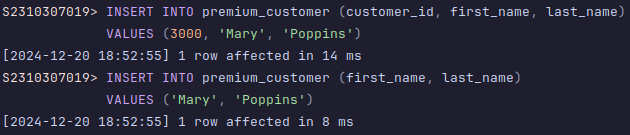
\includegraphics[width=0.8\textwidth]{../2_3_1.png}
	\caption{Ausgabe 2\textunderscore3\textunderscore1}
\end{figure}

\pagebreak

\begin{figure}[H]
	\centering
	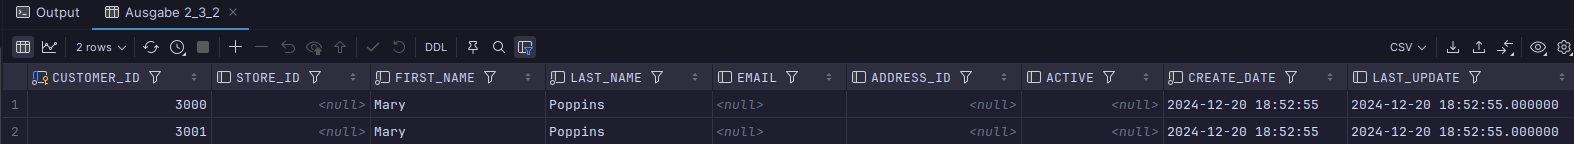
\includegraphics[width=1\textwidth]{../2_3_2.png}
	\caption{Ausgabe 2\textunderscore3\textunderscore2}
\end{figure}

\begin{figure}[H]
	\centering
	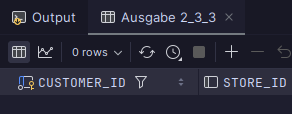
\includegraphics[width=0.4\textwidth]{../2_3_3.png}
	\caption{Ausgabe 2\textunderscore3\textunderscore3}
\end{figure}

\begin{figure}[H]
	\centering
	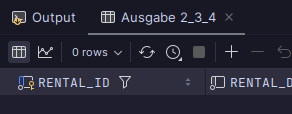
\includegraphics[width=0.4\textwidth]{../2_3_4.png}
	\caption{Ausgabe 2\textunderscore3\textunderscore4}
\end{figure}

\begin{figure}[H]
	\centering
	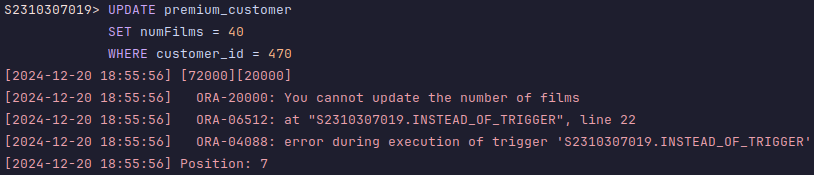
\includegraphics[width=0.8\textwidth]{../2_3_5.png}
	\caption{Ausgabe 2\textunderscore3\textunderscore5}
\end{figure}

\begin{figure}[H]
	\centering
	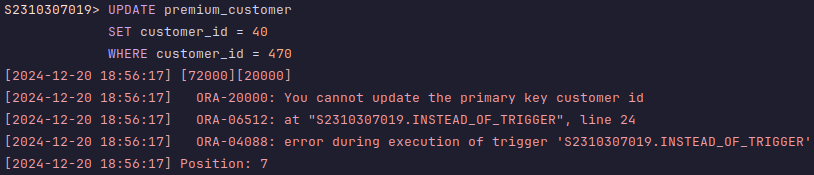
\includegraphics[width=0.8\textwidth]{../2_3_6.png}
	\caption{Ausgabe 2\textunderscore3\textunderscore6}
\end{figure}

\begin{figure}[H]
	\centering
	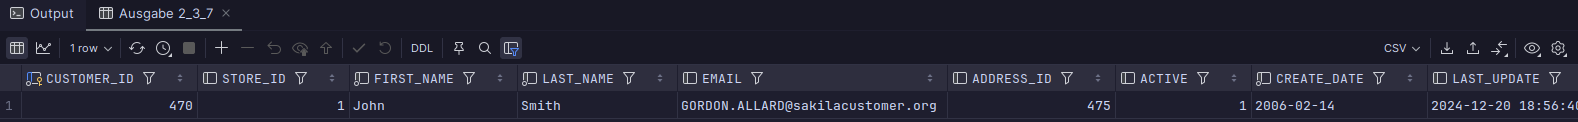
\includegraphics[width=1\textwidth]{../2_3_7.png}
	\caption{Ausgabe 2\textunderscore3\textunderscore7}
\end{figure}

\pagebreak

\section{Trigger für Systemereignisse}

\subsection{SQL-Statements}

\subsubsection{Aufgabe 1}
\inputminted{sql}{../ue5_3_1.sql}

\subsubsection{Aufgabe 2}
\inputminted{sql}{../ue5_3_2.sql}

\subsection{Ergebnisse}

\begin{figure}[H]
	\centering
	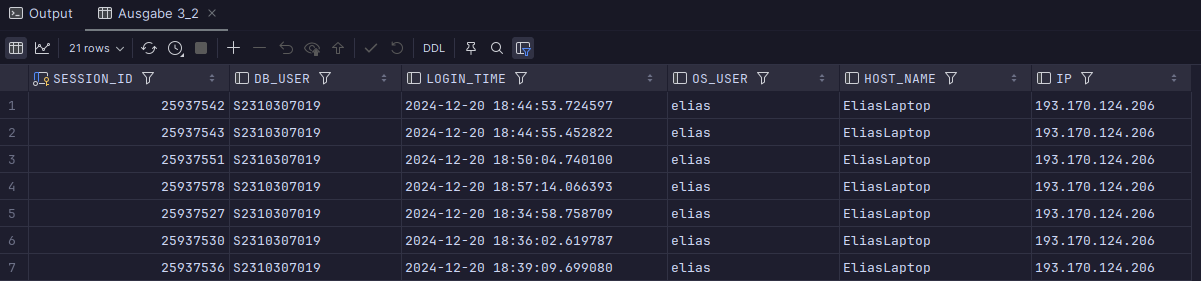
\includegraphics[width=1\textwidth]{../3_2.png}
	\caption{Ausgabe 3\textunderscore2}
\end{figure}

\end{document}